\documentclass{beamer}

\usetheme[hideothersubsections]{Berkeley}

% these are typical

\usepackage{latexsym}		% to get LASY symbols
\usepackage{epsfig}		% to insert PostScript figures
\usepackage{graphicx}           % to insert any other kind of figure

% these are for math stuff

\usepackage{amsmath}	% AMS math features (e.g., eqn alignment)
\usepackage{amssymb}	% Various weird symbols
\usepackage{amsfonts}	% Various useful math fonts
\usepackage{amsthm}	% Fancy theorem-type environments

% Uncomment these lines to make full-size pages for printing
%\usepackage{pgfpages}
%\pgfpagesuselayout{resize to}[letterpaper,border shrink=5mm,landscape]

% {definition}, {example}, {examples}, {lemma}, {theorem}, and {fact}
% already defined
\newtheorem{question}{Question}
\newtheorem{conjecture}{Conjecture}

\begin{document}

\raggedright

\title{A Question Answering System Using Encoder-decoder Sequence-to-sequence Recurrent Neural Networks}
\author{Bo Li}
\date{May, 2018}
\institute[SJSU]{San Jos\'{e} State University}

\begin{frame}
\titlepage

\end{frame}

\begin{frame}

  \frametitle{Outline}

  \tableofcontents[hideallsubsections]

\end{frame}



\section{Introduction}

\begin{frame} \frametitle{Question Answering}
    \begin{itemize}
        \item the study of writing computer programs that can answer natural language questions
        \item are widely used among search engines, personal assistant applications on smart phones, voice control systems and various other applications
        \item  can be categorized into two types - open domain and close domain
    \end{itemize}
\end{frame}

\begin{frame}{Open Domain \& Close Domain}
    For an open domain system, the questions can be about almost everything; whereas, for a close domain system, the questions are about a specific domain.
\end{frame}

\begin{frame}{Topic of This Project}
    \begin{itemize}
        \item open domain
        \item a scenario where a specific passage is assigned to a question and the answer is a segment of the passage
        \item The Stanford Question Answering Dataset (SQuAD) used in this project is appropriate for such scenario
    \end{itemize}
\end{frame}

\begin{frame}{Stanford Question Answering Dataset (SQuAD)}
    \begin{itemize}
        \item includes questions asked by human beings on Wikipedia articles
        \item The answer to each question is a segment of the corresponding Wikipedia passage
        \item contains more than 100,000 question-answer pairs on more than 500 articles
    \end{itemize}
\end{frame}
\begin{frame}{Encoder-decoder Sequence-to-sequence Recurrent Neural Networks}
   \begin{itemize}
       \item These networks encode an input sequence to some vectors and then decode them to an output sequence. \item For question answering, the input sequence includes a passage and a question and the output sequence is the answer
   \end{itemize}
\end{frame}

\begin{frame}{Contribution of This Project}
    \begin{itemize}
        \item successfully built a question answering system using five different models
        \item By comparing the results of five different models, we got two interesting observations
    \end{itemize}
\end{frame}

\section{Background}

\begin{frame} \frametitle{Word Feature Vector}
  \begin{itemize}
      \item A word feature vector represents a word according to its relationship with other words in a vocabulary.
      \item The distance from one word feature vector to any other word feature vector tells how likely the two words appear in a same context.
      \item The word feature vector matrix for the vocabulary of a given text are learned by training a neural probabilistic language model on the text

  \end{itemize}
\end{frame}

\begin{frame}{Word Feature Vector, cont.}
    neural probabilistic language model
    \begin{itemize}
        \item Denote V as the vocabulary, $w_t$ as a word from $V$, and the matrix $C$ as the word feature vectors of all words in $V$.
        \item Each instance of the training set is a sequence of words $w_1,...,w_T$ which is a segment of the text.
        \item The purpose of a neural probabilistic language model is to learn a model $f$ such that
        $$ f(w_t, ..., w_{t-n+1}) = \hat{P}(w_t | w_{t-1},...,w_{t-n+1}).$$

    \end{itemize}
\end{frame}

\begin{frame}{Word Feature Vector, cont.}
    neural probabilistic language model
    \begin{itemize}
        \item The computation of $f(w_t, ..., w_{t-n+1})$ is divided into two parts:
            \begin{itemize}
                \item First, each $w$ is mapped to a word feature vector by selecting the corresponding row in $C$ to get

                $$x=(C(w_{t-1}),... ,C(w_{t-n+1})).$$

                \item Second, we get $f(w_t, ..., w_{t-n+1})$ through

                $$y=b+W\cdot x + U\cdot tanh(d + H\cdot x)$$

                and

                $$ f(w_t, ..., w_{t-n+1}) = \frac{e^{y_{w_t}}}{\sum_{i}^{}e^{y_i}}.$$
            \end{itemize}
        \item The loss function to minimize is $$L = -\frac{1}{T}\sum _{t}^{} \log{f(w_t, ..., w_{t-n+1})}.$$
    \end{itemize}
\end{frame}

\begin{frame}{Word Feature Vector, cont.}
   \begin{itemize}
       \item In the neural probabilistic language model, the word feature vectors are used to predict the next word after a sequence. However, the usage of word feature vectors is far beyond this.
       \item Using word feature vectors to represent words is common when applying neural network models on natural language processing tasks. This is how we used word feature vectors in this project.
   \end{itemize}

\end{frame}
\begin{frame}{Recurrent Neural Networks}

Recurrent Neural Networks (RNNs) are used for modeling sequential data

    \begin{examples}{A simple recurrent network with no outputs}
        \begin{itemize}
            \item $x$ is the input. $h$ is the state. $\theta$ is the hyperparameter.
            \item The relation between $h$ and $x$ is
            $$h_t = f(h_{t-1}, x_t; \theta).$$

            \item An example of $f$ is

            $$h_t = sigmoid(W_h h_{t-1} + W_x x_t + b).$$
        \end{itemize}
    \end{examples}

\end{frame}

\begin{frame}{Recurrent Neural Networks, cont.}
    \begin{center}
      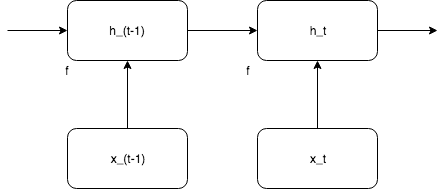
\includegraphics[width=9cm, height=3cm]{figures/rnnWithNoOutputs}
    \end{center}
\end{frame}

\begin{frame}{Recurrent Neural Networks, cont.}
    \begin{itemize}
        \item the vanishing gradient problem exists
            \begin{itemize}
                \item the vanishing gradient means the gradients become smaller and smaller as their values are propagated forward in a network
                \item When this happens, the network learns slowly or even stops learning
            \end{itemize}
        \item The main solution to the vanishing problem is to use a more complex learning unit
        \item Long Short Term Memory (LSTM) cell is one such complex learning unit; Gated Recurrent Unit (GRU) has a simplified structure but similar function with LSTM
        \item In this project, I used LSTM and GRU equally as learning unit
    \end{itemize}
\end{frame}

\begin{frame}{Bidirectional Recurrent Neural Networks}
    \begin{itemize}
        \item Problem of RNNs: $h_t$ only contains context information from $x_1$ to $x_t$
        \item Solution given by Bidirectional RNNs:
        \begin{itemize}
            \item one cell operates from left to right, and another cell operates from right to left
            \item using both $h_t$ and $g_t$ can get context information of the whole sequence
        \end{itemize}
    \end{itemize}

    \begin{center}
        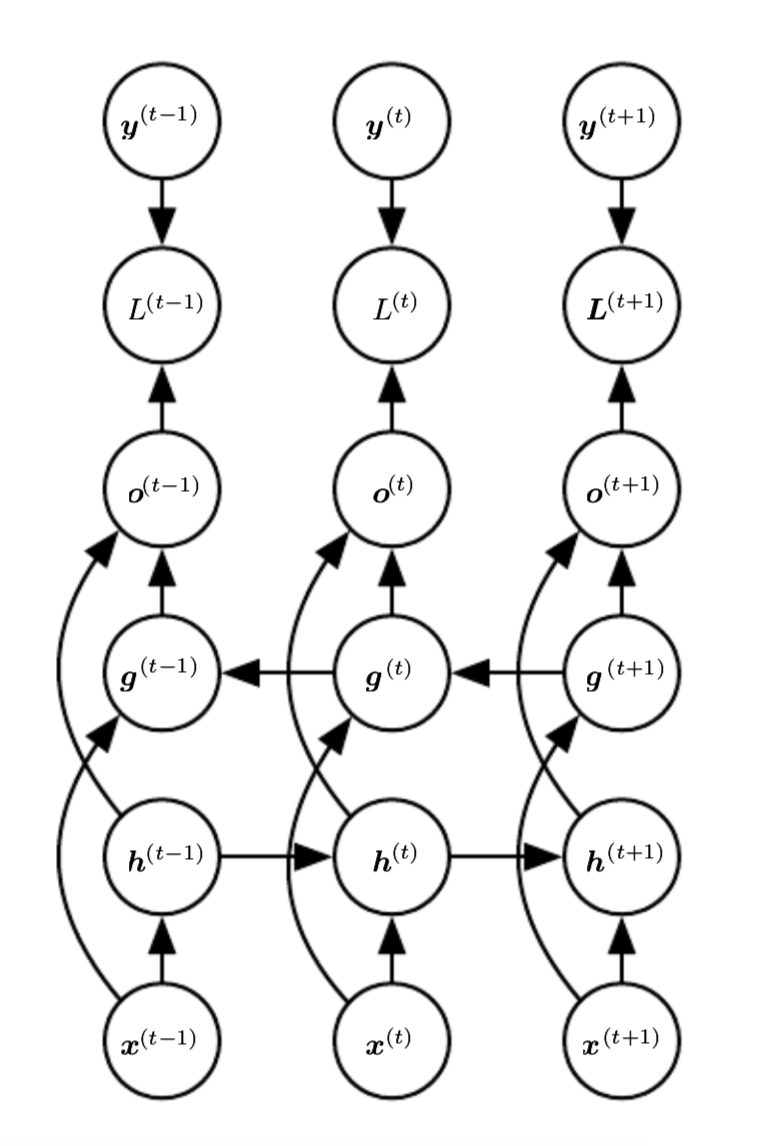
\includegraphics[width=8cm, height=5cm]{figures/bidirectionalRnn.png}
    \end{center}

\end{frame}

\begin{frame}{Encoder-decoder Sequence-to-sequence Architecture}
\begin{itemize}
    \item The process of understanding the input sequence is considered as encoding the input sequence to some vectors $Crypto$.
    \item The process of generating output is considered as decoding the $Crypto$.
\end{itemize}

\begin{examples}
$x$ is the input, $h$ is the state in encoding process, $y$ is the output, and $g$ is the state of decoding process.
\end{examples}

\end{frame}

\begin{frame}{Encoder-decoder Sequence-to-sequence Architecture, Cont.}
    \begin{center}
        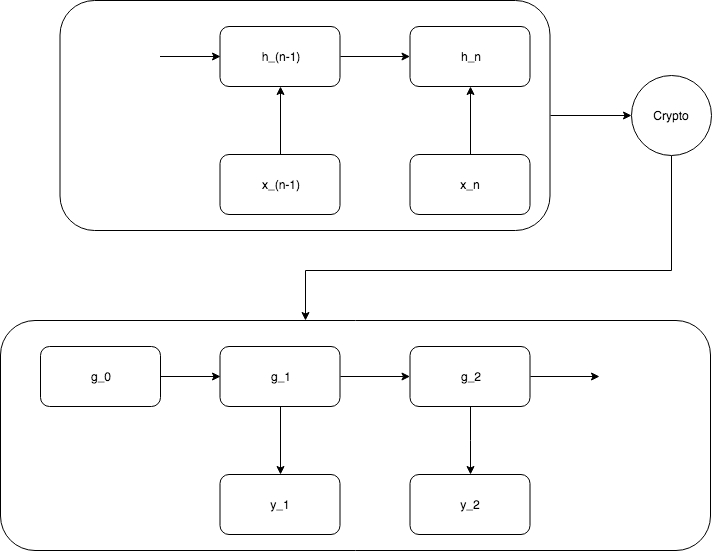
\includegraphics[width=10cm, height=7cm]{figures/encoderDecoder.png}
    \end{center}
\end{frame}

\begin{frame}{Encoder-decoder Sequence-to-sequence Architecture, Cont.}
    \begin{itemize}
        \item The question answering task in this project is a sequence-to-sequence task.
        \item Each input actually includes two sequences - a question and a passage.
            \begin{itemize}
                \item attention mechanism is required to make each passage aware of the corresponding question and encode the two together
            \end{itemize}
        \item each output sequence is an answer which is represented by two indices for the input passage sequence.
            \begin{itemize}
                \item pointer network is required to make sure the output sequence comes from input sequence
            \end{itemize}
    \end{itemize}

\end{frame}

\begin{frame}{Attention Mechanism}
    \begin{itemize}
        \item first used in neural machine translation
        \item is used to enable the decoding process aware of the encoding states
    \end{itemize}
\end{frame}

\begin{frame}{Attention Mechanism, Cont.}
    \begin{examples}
        $y$ is the output, $g$ is the state, and $c$ is the attention vector. $$g_i =f(g_{i-1},y_{i-1},c_i).$$
        The attention vector $c_i$ is produced by using $g_{i-1}$ to ``query'' the encoding states $h_1, ... h_n$ through
        $$c_i = \sum _j {\alpha _{i,j} h_j}$$
        $$\alpha _{i,j} = \exp{e_{i,j}} / \sum _j {\exp{e_{i,j}}}$$
        $$e_{i,j} = tanh(W_h h_j + W_g g_{i-1} + b).$$
    \end{examples}

\end{frame}

\begin{frame}{Attention Mechanism, Cont.}
    \begin{center}
        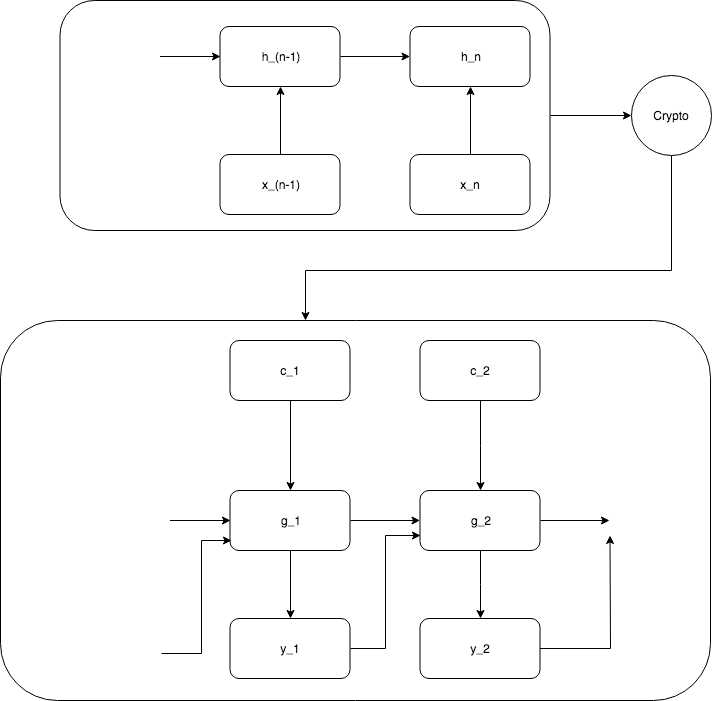
\includegraphics[width=8cm, height=8cm]{figures/attention}
    \end{center}
\end{frame}

\begin{frame}{Attention Mechanism, Cont.}
    In this project, the passage is required to ``be aware of the question'' in encoding process. At the same time, the answer is required to ``be aware of the encoding states of passage and question''. The detailed formulas are given later.
\end{frame}

\begin{frame}{Pointer Network}
    \begin{itemize}
        \item Using the pointer network enables the decoder to output tokens from input sequence
        \item The attention mechanism is used with the pointer network
        \item However, aside from getting an attention vector, the attention weight vector $\alpha$ is considered as a probability distribution which indicates how likely each token in the input sequence is the current output.
        $$y_i = x_k$$
        where
        $$k = argmax_j(\alpha _{i,j}).$$
    \end{itemize}
\end{frame}

\begin{frame}{Pointer Network, Cont.}
    \begin{center}
        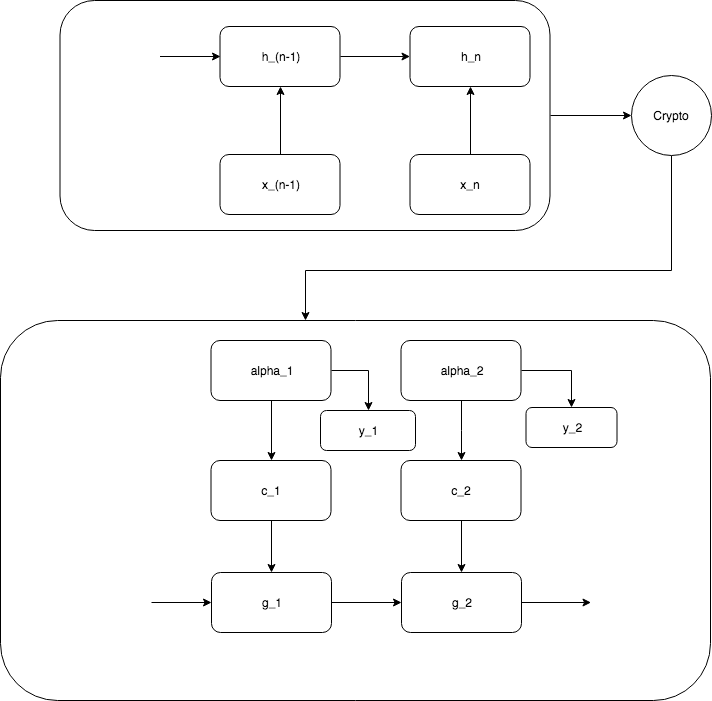
\includegraphics[width=8cm, height=8cm]{figures/pointerNetwork.png}
    \end{center}

\end{frame}

\begin{frame}{Pointer Network, Cont.}
    In this project, the pointer network was used in the decoding part of several models.
\end{frame}
\section{Design}

\begin{frame} \frametitle{Model 1}

\end{frame}

\begin{frame} \frametitle{Model 2}

\end{frame}

\begin{frame} \frametitle{Model 3}

\end{frame}

\begin{frame} \frametitle{Model 4}

\end{frame}

\begin{frame} \frametitle{Model 5}

\end{frame}

\section{Implementation}

\begin{frame} \frametitle{Adjusting Models for Batch Training}

\end{frame}


\begin{frame}{Tensorflow Graphs}

\end{frame}

\begin{frame}{Implementation Pipeline}

\end{frame}

\section{Experiments}

\begin{frame} \frametitle{Data}

\end{frame}

\begin{frame}{Settings}

\end{frame}

\begin{frame}{Training Process}

\end{frame}

\begin{frame}{Testing Results}

\end{frame}

\begin{frame}{Analysis}

\end{frame}

\section{Conclusion}

\begin{frame}{Contribution of This Project}

\end{frame}

\begin{frame} \frametitle{Future Work}

\end{frame}

\begin{frame}
Thank you! Questions?
\end{frame}

\end{document}
